
En el tejado con ángulo de inclinación $\varphi$ yace una hoja de plomo. El coeficiente de fricción del plomo con el tejado $\mu\gg tg(\varphi)$. El coeficiente de dilatación lineal del plomo es $\alpha$. La longitud de la hoja a temperatura mínima \textit{t}$_1$, es igual a \textit{l}. Considerando que la temperatura durante el día sube, alcanzando el valor máximo \textit{t}$_2$ y luego baja de nuevo hasta \textit{t}$_1$, hállese el punto inmóvil, tanto para el caso en que la hoja se calienta, como para el que se enfría. ¿A qué distancia se desplazará la hoja durante $N$ días, siendo el tiempo estable?

\begin{figure}[h!]
    \centering
    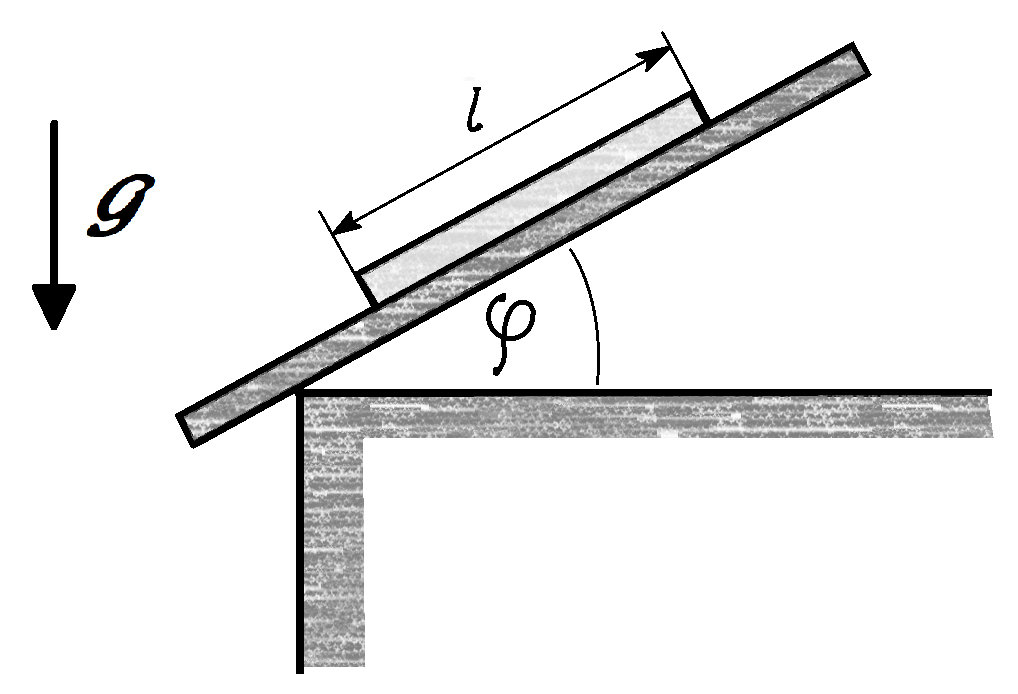
\includegraphics[scale=0.23]{f_savchenko_p35_2-1-28.png}
    \caption{Problema 6}
\end{figure}